\documentclass[a4paper,12pt,twoside,english,openany]{book}
\usepackage[icon=Note,color=yellow,author=Sepand]{pdfcomment}
\usepackage[utf8]{inputenc}
\usepackage[figuresright]{rotating}
\usepackage[T1]{fontenc}
\usepackage{babel}
\usepackage[a4paper,left=3cm,right=2.5cm,top=3cm,bottom=3cm, twoside]{geometry}
\usepackage{xcolor}
\usepackage{stmaryrd}
\usepackage{amssymb}
\usepackage{amsmath}
\usepackage{libertine}
\usepackage[
    natbib=true,
    style=numeric,
    sorting=none,
    maxcitenames=1,
]{biblatex}

\addbibresource{res/biblio.bib} 
\addbibresource{res/biblio2.bib} 

\usepackage[font=small,labelfont=bf]{caption}
\usepackage{subcaption}
\usepackage{float}
\usepackage{multirow}
\usepackage[Export]{adjustbox}
\usepackage{array, multirow, tabularx}
\usepackage{booktabs}
\usepackage{longtable}
\usepackage{setspace}
\usepackage{apalike}
\usepackage{minitoc}
\usepackage{tikz}
\usetikzlibrary{calc, positioning, arrows.meta,arrows, shapes.geometric,backgrounds}
\usepackage[strict]{changepage}
\usepackage{siunitx}
\usepackage{enumitem}
\usepackage{epigraph}
\usepackage{lscape}
\usepackage{titletoc}
\usepackage{mdframed}
\usepackage{tabu}
\usepackage{pdfpages}
\usepackage{arydshln}
\usepackage{titling}
\usepackage{calc}
\usepackage[xindy]{imakeidx}
\usepackage{upgreek}
\usepackage{titlesec} 
\usepackage{sectsty}
\usepackage{lipsum}
\usepackage{emptypage}
\usepackage{fancyhdr}
\pagestyle{fancy}
\usepackage{graphicx}
\graphicspath{ {res/} }
\usepackage{hyperref} 
\hypersetup{
    colorlinks=true,
    linkcolor=black,
    filecolor=black,      
    urlcolor=black,
    citecolor=black,
    }
\definecolor{linkColor}{HTML}{32a852}

\titleformat{\chapter}[hang]
  {\normalfont\bfseries}{}{0pt}{\Huge}

\makeatletter
\renewcommand\section{%
  \@startsection{section}{1}{\z@}
  {1.5ex plus .2ex minus .2ex}
  {0.6ex}%                      
  {\normalfont\Large\bfseries}}

\renewcommand\subsection{%
  \@startsection{subsection}{2}{\z@}%
  {1.2ex plus .2ex minus .2ex}
  {0.5ex}
  {\normalfont\large\bfseries}}

\renewcommand\subsubsection{%
  \@startsection{subsubsection}{3}{\z@}%
  {0.5ex plus .2ex minus .2ex}
  {0.5ex}
  {\normalfont\normalsize\bfseries}}
\makeatother
\title{Estimation of Image-Derived Arterial Input Function in Brain PET Imaging: \\ Application to Modeling PET Dynamics of Glucose Metabolism in Patients with Impaired Consciousness}

\author{Sepand Ali Madad Soltani}
\date{March 2025}



\leftmark 
\rightmark 


% \makeindex
%\input{auxilliaires/glossaire}
\def\mrglu{\text{MR}_{\text{glu}}}
\newcommand{\fdg}{$[^{18}\mathrm{F}]\text{FDG}$}
\newcommand{\yohimbine}{$[^{11}\mathrm{C}]\text{Yohimbine}$}
\newcommand{\sym}[1]{\textsuperscript{#1}}


\begin{document}

\begin{titlepage}
	\begin{center}
		\begin{tabular}{c@{\hskip 7cm}c@{\hskip 1cm}}
			
\includegraphics[height=3cm]{res/ucbl.png} &
			
\includegraphics[height=3cm]{res/polytech2.png}
			% 
\includegraphics[width=5cm]{res/cermep.png}
		\end{tabular}
	\end{center}

	\begin{center}

		\vspace*{.03\textheight}
		\textsc{\Large University of Claude Bernard Lyon 1}\\[0.2cm]
		\large Polytech Lyon

		\rule{\textwidth}{0.8pt} \\
		\vspace{10pt}

		{\huge \bfseries \thetitle}
		\rule{\textwidth}{0.8pt} \\

		\vfill

		\vspace{18mm}

		{\Large \textsc{Sepand Ali Madad Soltani}}\\[3mm]
		{\large Master 2 in Medical Device Engineering}\\[1mm]
		{\large Internship Report}

		\vspace{12mm}

		{\normalsize \textit{Supervised by} \textsc{Inés Merida} \textit{and} \textsc{Nicolas Costes}}\\[2mm]
		{\normalsize \textit{Academic Advisor} \textsc{Kevin Tse-Ve-Koon}}

		\vspace{10mm}

		{\normalsize \textit{Hosting Laboratory}}\\
		{\normalsize CERMEP- imagrie du vivant, Bron, France}

		\vfill

		{\large 2024--2025}
		%
		%
		% \vfill
		% By \textsc{\Large Sepand Ali Madad Soltani}\\
		% Master 2 in Medical Device Engineering \\
		% Internship Report\\
		% Supervised by \textsc{\large Inés Mérida} and \textsc{\large Nicolas Costes}  \\
		% Academic Advisor: \textsc{\large Kevin Tse Ve Koon}\\
		% Hosting Laboratory:\\
		% CERMEP - Imagrie du Vivant, Lyon, France\\
		% 2024-2025
		%
	\end{center}

	\vspace{1cm}
\end{titlepage}

\renewcommand{\chaptermark}[1]{\markboth{#1}{}}


\frontmatter
\chapter*{Abstract}
\addcontentsline{toc}{chapter}{Abstract}
Dynamic PET quantification requires an arterial input function (AIF), but arterial sampling is invasive.
Image-derived input functions (IDIFs) offer a non-invasive alternative, yet accurate segmentation of arteries and partial volume effects (PVE) limit accuracy.
We present an automatic pipeline that segments the internal carotid arteries on TOF-MRA and estimates an IDIF with a Bayesian Geometric Transfer Matrix (BGTM) model.
The model uses a population-informed PCA prior for the input function, a spectral model for background tissue, and frame-wise weights to account for time-varying noise.
We evaluated the approach on two experimental cohorts: comatose patients with an injection of \fdg\ and healthy adults with an injection of \yohimbine.
In the \fdg\ dataset, BGTM improved quantitative accuracy over GTM and a population-based input function (PBIF), reducing \(\mrglu\) error on average (mean MAPE 13\% vs 24\% for GTM and 17\% for PBIF).
In the \yohimbine\ dataset, BGTM lowered the large errors seen with GTM but did not surpass PBIF (mean \(V_T\) MAPE 75.9\% vs 166.5\% and 29.5\%).
Performance was likely affected by the small PCA sample and by subject motion.
We also conducted Monte Carlo PET simulations as complementary validation under controlled conditions, with known ground truth.
Simulations reproduced realistic brain activity but showed a systematic underestimation of arterial activity relative to the prescribed input.
Indicating the need for a more rigorous simulation design in future studies
These results show that non-invasive IDIF is feasible with multimodal PET--MR and principled treatment of PVE and noise, with clear gains for \fdg\ and potential for higher accuracy for other tracers as well.
\paragraph{Keywords:} Dynamic FDG-PET, Image-Derived Input Function, Hybrid PET/MRI, Bayesian Framework


\tableofcontents

\mainmatter
\setlength{\parskip}{.7em}

\renewcommand{\baselinestretch}{1.1}


\fancyhead[]{}
\fancyfoot[]{}
\fancyhead[LH]{\leftmark}
\fancyhead[RH]{\thepage}


\chapter{Introduction}

\section{Positron Emission Tomography}
% GPT: dont touch
Positron Emission Tomography (PET) is an in vivo functional imaging technique widely used in clinical and research settings to monitor physiological and biochemical processes.
In PET, a biologically active molecule is labeled with a positron-emitting radioisotope, serving as a radiotracer, and then injected into the body.
As the radiotracer accumulates in target tissues, its radioactive decay produces positrons, which interact with electrons to emit pairs of gamma photons in nearly opposite directions.
These photons are detected by the PET scanner, and image reconstruction algorithms generate a three-dimensional representation of the tracer distribution.
This imaging modality allows for the investigation of metabolic changes, receptor binding, and other biochemical processes, providing invaluable information in oncology, neurology, cardiology, and other fields.

There are two main categories in PET image acquisition: static imaging and dynamic imaging.
Static PET involves acquiring a single scan after the radiotracer injection.
This single snapshot offers a powerful yet simplified view of tracer distribution.
The common quantification metric in static imaging is the Standardized Uptake Value (SUV), which normalizes tissue uptake by the injected dose and weight of the subject, allowing for a semi-quantitative comparison of tracer accumulation across different tissues or over time \cite{keyes1995suv}.
Due to its simplicity, static PET is widely used in clinical settings; however, it also has limitations.
Because it reflects only one time point, the SUV cannot capture the temporal dynamics of tracer uptake and clearance, and various physiological factors may influence its measurements, thereby reducing its accuracy.

Dynamic PET imaging provides a more comprehensive view of radiotracer kinetics by acquiring a series of images over a period ranging from a few minutes to more than an hour post-injection, depending on the tracer type.
Instead of a single snapshot, dynamic imaging produces time-activity curves (TAC) that illustrate how tracer concentration in each tissue changes throughout the scanning period.
This approach enables the measurement of physiological parameters such as the tracer rate of influx (\(K_i\)) for radiotracers with irreversible uptake (e.g. \fdg ), volume of distribution (\(V_T\)), and the rates of phosphorylation and dephosphorylation.

\section{Kinetic Modeling}
% GPT: dont touch
To quantify pharmacokinetic parameters, kinetic modeling is employed.
Compartmental modeling is the most popular and is considered the most accurate approach in kinetic modeling.
In compartmental modeling, the distribution and kinetics of a radiotracer are described by dividing the system into distinct compartments, each representing a pool of tracer that behaves uniformly.
Interactions between compartments can be unidirectional or bidirectional, meaning the tracer may either move in and out or only enter a compartment.
Various graphical models (e.g., the Logan \cite{logan1990graphical} and Patlak \cite{patlak1983graphical} methods), as well as classical compartmental model fitting approaches, are used to analyze tracer kinetics.

Figure~\ref{fig:2tcm} shows the two-tissue compartment model (2TCM), also known as the three-compartment model, in series mode.
This model comprises one tissue compartment for the free tracer, \(C_F(t)\), and another for the receptor-bound tracer, \(C_B(t)\), in addition to an external compartment representing the tracer concentration in the plasma or blood, denoted as the input function \(C_P(t)\).

The tracer kinetics are governed by a series of first-order differential equations, in which the exchange rates between the compartments are considered constant:
\begin{align}
	\frac{dC_F(t)}{dt} & = K_1 \, C_P(t) \;-\; \bigl(k_2 + k_3\bigr) C_F(t) \;+\; k_4 C_B(t) \,, \label{eq:2tcm-c1} \\[6pt]
	\frac{dC_B(t)}{dt} & = k_3 \, C_F(t) \;-\; k_4 \, C_B(t), \label{eq:2tcm-c2}
\end{align}
where \(K_1\), \(k_2\), \(k_3\), and \(k_4\) are the constant rate parameters.

\begin{figure}[b]
	\centering
	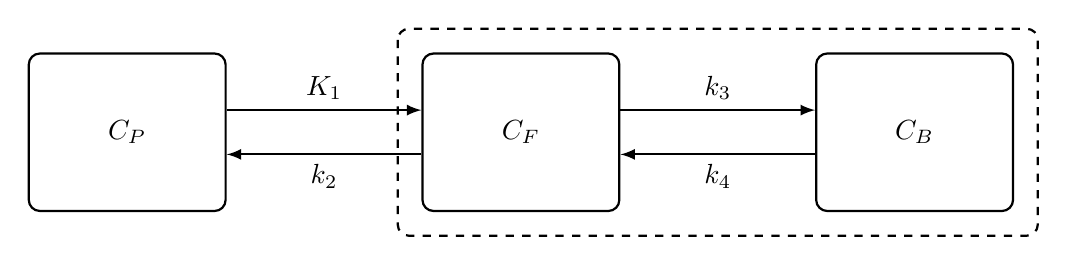
\begin{tikzpicture}[>=latex, thick]
		\node[draw, rounded corners, minimum width=2.5cm, minimum height=2cm, align=center] (Cp) at (0,0) {$C_P$};
		\node[draw, rounded corners, minimum width=2.5cm, minimum height=2cm, align=center] (C1) at (5,0) {$C_F$};
		\node[draw, rounded corners, minimum width=2.5cm, minimum height=2cm, align=center] (C2) at (10,0) {$C_B$};

		\draw[->]
		([yshift=8pt]Cp.east) to[out=0, in=180]
		node[above] {\(K_1\)}
		([yshift=8pt]C1.west);

		\draw[->]
		([yshift=-8pt]C1.west) to[out=180, in=0]
		node[below] {\(k_2\)}
		([yshift=-8pt]Cp.east);

		\draw[->]
		([yshift=8pt]C1.east) to[out=0, in=180]
		node[above] {\(k_3\)}
		([yshift=8pt]C2.west);

		\draw[->]
		([yshift=-8pt]C2.west) to[out=180, in=0]
		node[below] {\(k_4\)}
		([yshift=-8pt]C1.east);

		\draw[dashed, rounded corners, thick] ($(C1.north west)+(-0.3,0.3)$) rectangle ($(C2.south east)+(0.3,-0.3)$);

	\end{tikzpicture}
	\caption{Schematic of the two-tissue compartment model (2TCM)}
	\label{fig:2tcm}
\end{figure}

The total radiotracer tissular kinetic measured by PET (the PET data), \(C_T(t)\), is given by
\begin{equation}
	C_T(t) \;=\; C_F(t) \;+\; C_B(t) \;+\; C_P(t).
\end{equation}

Thus to solve this system of equations and to estimate \(K_1\), \(k_2\), and \(k_3\) parameters, we must fit the model using the measured PET TACs ($C_T$) and the input function ($C_P$).

For \fdg$\,$ quantification, the metabolic rate of glucose (\(\textrm{MR}_{\textrm{glu}}\)) is calculated as
\begin{equation}
	\textrm{MR}_{\textrm{glu}} \; (\textrm{\textmu mol/min/100g}) = \frac{[C]}{LC} \cdot \frac{K_1 \times k_3}{k_2 + k_3} \,.
\end{equation}
where \([C]\) denotes the glucose concentration, and \(LC\) is the lumped constant.

For \yohimbine $\,$ quantification, we utilize the Volume of Distribution ($V_T$) which is the ratio of radiotracer concentration in the target tissue ($C_T$) to the plasma ($C_P$):
\[
	V_T = \frac{C_T}{C_P}
\]

Using the Logan plot method this can be directly estimated from these two values or to be fitted to a compartment model.
In the latter case, $V_T$ can be calculated as
\[
	V_T = \frac{K_1}{k_2} (1+\frac{k_3}{k_4})
\]

\section{Input Function}

\subsection{Arterial Input Function}
% GPT: Dont change
The arterial input function (AIF) is considered the gold standard for obtaining the input function.
It is determined by inserting an arterial catheter into the patient and continuously drawing blood samples to measure the radiotracer concentration, thereby obtaining the blood activity curve used in the quantification model.
However, this procedure is invasive and can cause discomfort, potentially discouraging patients from undergoing future examinations.
Furthermore, this method is labor-intensive and requires trained personnel to manage both the subject and the measurement devices.

\subsection{Population-Based Input Function}
Population-Based Input Function (PBIF) is a method for replacing the subject specific AIF with the average AIFs of a population of other subjects.
% GPT: explain a bit more, max 1-2 sentences
In practice, an average curve is derived from a representative cohort and then temporally aligned and scaled to the subject using one or more calibration points (e.g., early blood samples or image-derived peaks).
PBIF can reduce invasiveness and acquisition burden, but it may introduce bias if the cohort is not well matched to the subject or if calibration is suboptimal.

\subsection{Image Derived Input Function}
% GPT: Dont change
The image-derived input function (IDIF) has been proposed as a non-invasive alternative for obtaining the input function.
IDIF techniques typically involve identifying vascular structures or regions with high blood pool activity within the imaging field and extracting the input function directly from the PET images.
For example, in whole-body, cardiac or small animal PET studies the aorta is visible in the in the Field of View (FOV) of the PET camera and is used as the source for IDIF.
In brain PET imaging, the Internal Carotid Arteries (ICA) are the largest vessels present in the FOV and have a diameter of approximately 5 mm much smaller than of the aorta.
Their smaller size makes IDIF more challenging due to Partial Volume Effects

\section{Partial Volume Effect}
% GPT: explain PVE in a few lines.
Partial Volume Effect (PVE) is
the loss and mixing of signal that occurs when structures are small relative to the system’s spatial resolution, causing activity to “spill out” of small objects and “spill in” from neighbors.
In PET, this leads to systematic underestimation of arterial activity and contamination from surrounding tissue, especially for vessels like the ICA that have similiar size as the effective resolution of PET camera (both around 5mm).
In Figure~\ref{TODO}, this effect is shown [TODO]
Correcting PVE is essential for accurate IDIF estimation and downstream kinetic modeling.

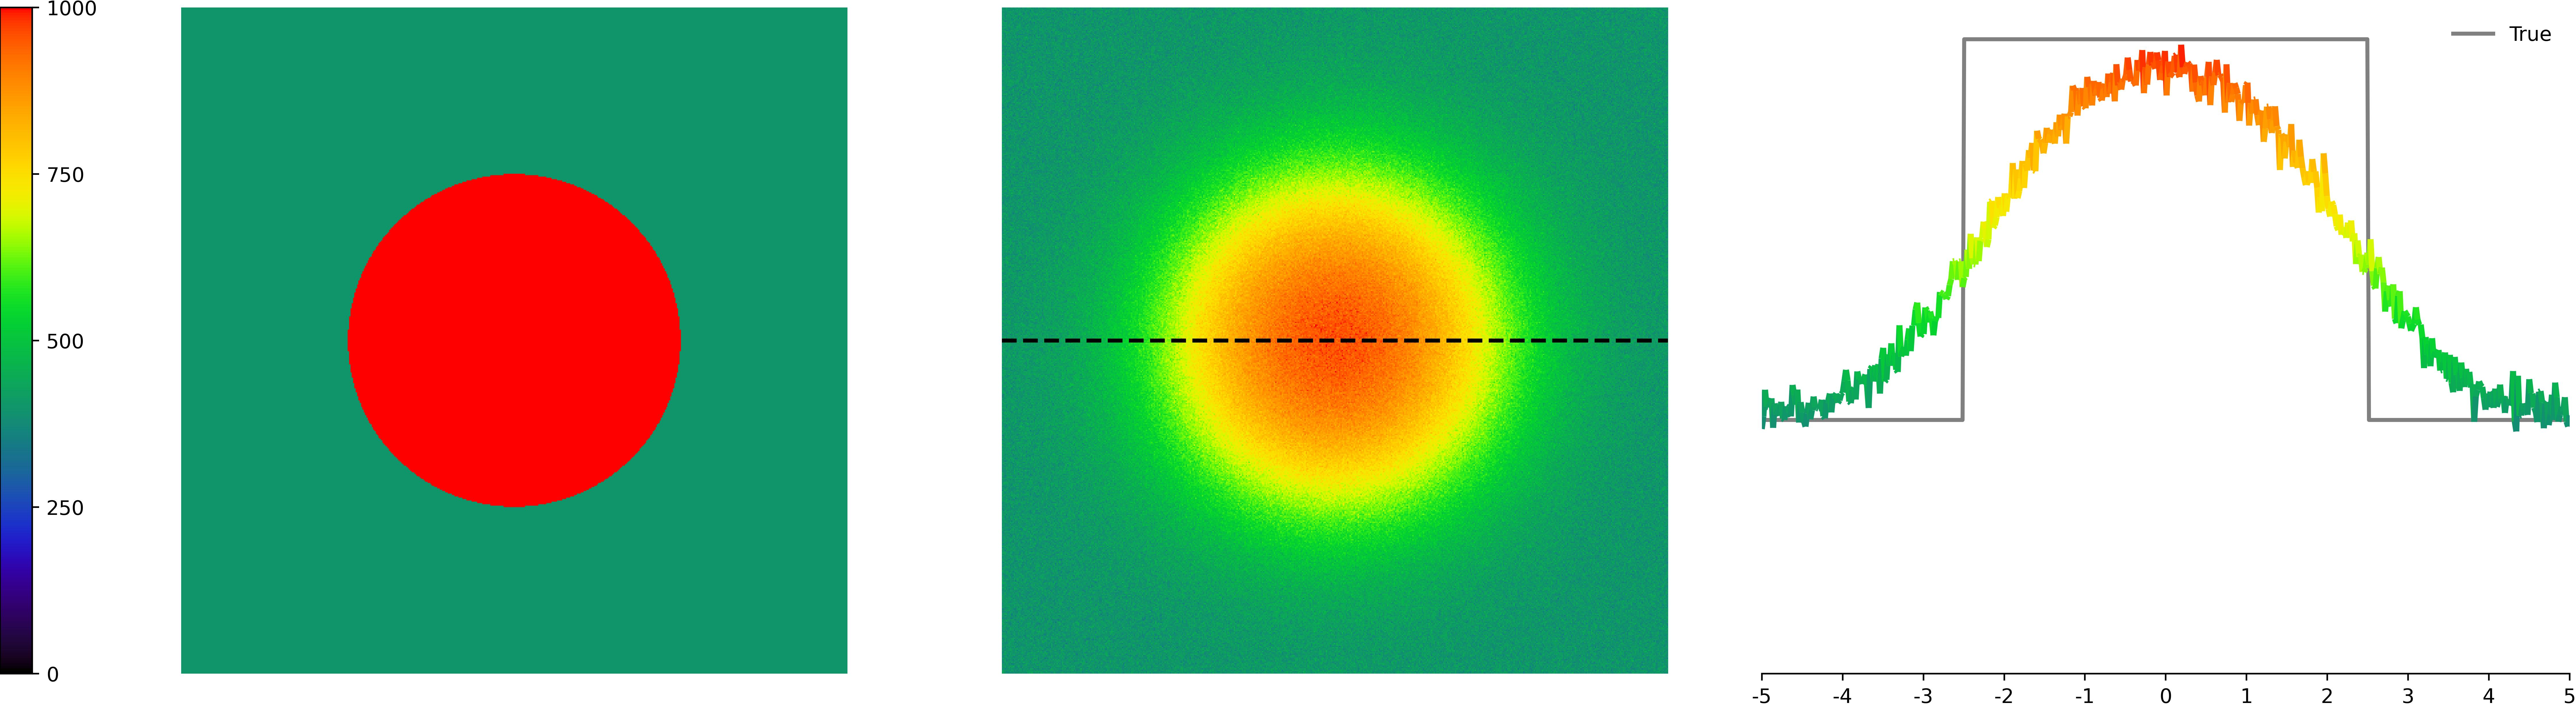
\includegraphics[width=\textwidth]{figures/pve.jpg}
\section{Background}
% GPT: improve sentencing and add slightly more description to some methods that i didnt explain enough
Many methods have utilized the first few frames of the dynamic PET, when the tracer has not yet reached tissue and predominantly resides in the arteries, to obtain a mask of the carotids \cite{young2023image}.
These implementations range from fully manual approaches \cite{TODO}, to semi-automatic methods that use a few seed voxels for region growing or to initialize morphological operations \cite{TODO}, and to fully automatic pipelines based on deep learning such as custom Convolutional Neural Networks (CNNs) \cite{TODO} and U-Net architectures \cite{TODO}.

However, even with sophisticated approaches, ICA segmentation directly from PET suffers from strong PVE.
With the emergence of hybrid PET/MRI systems, it has become feasible to acquire both functional and anatomical data simultaneously.
MRI provides high-resolution soft-tissue contrast, while PET captures metabolic activity.
For instance, time-of-flight MR angiography (TOF-MRA) delivers excellent arterial contrast.
Many studies have leveraged this to achieve accurate ICA segmentation using manual or semi-automatic procedures, typically relying on high-intensity thresholding and seeded or unseeded region growing \cite{TODO}.


Unlike T1-weighted MRI, TOF-MRA is not always included in research and clinical protocols.
Meanwhile, T1-weighted scans are routinely acquired for anatomical localization and image registration, among other purposes, which makes them a practical source for arterial segmentation when TOF-MRA is not part of the protocol.
In this context, \citeauthor{TODO} \cite{TODO} proposed a deep learning model that infers the ICA directly from T1-weighted images.
Similarly, the caliPER software \cite{TODO} enables semi-automatic extraction of arterial masks from either TOF-MRA or T1-weighted data.


As noted above, even with a high-resolution anatomical arterial mask, PVE remains and must be corrected.
Partial Volume Correction (PVC) methods estimate spill-in and spill-out coefficients between the ICA and surrounding tissue.
Recovery Coefficients (RC) are commonly used, obtained by scanning cylindrical phantoms of various diameters and matching the ICA diameter to the closest phantom \cite{TODO,TODO,TODO,TODO}.
The Geometric Transfer Matrix (GTM) method generalizes this by estimating regional spillover based on volume geometry and an explicit point spread function (PSF) model \cite{TODO}.
However, these linear mixing models do not account for additional effects such as time-varying noise or motion, and they typically treat the problem as a fixed linear unmixing (\(\text{SP}\cdot C_{\text{in}} - \text{SO}\cdot C_{\text{out}}\)) without propagating uncertainty, which can limit recovery in challenging conditions.

More advanced approaches include model-based matrix factorization that jointly estimates the input function and tissue activity \cite{TODO}, as well as deep learning methods trained to infer the IDIF from PET and MRI inputs \cite{TODO,TODO}.

In this work, we propose a fully automatic pipeline for extracting the ICA mask from TOF-MRA.
We then employ a Bayesian framework that couples GTM-based mixing with priors on the input function and tissue kinetics, explicitly modeling noise to improve IDIF estimation \cite{irace2021bayesian}.


\chapter{Materials and Methods}

\section{Dataset Description}
Two experimental datasets were available.
In the first study, 59 acute comatose patients were included between 7 days and 30 days after coma onset (46 ± 16 years old; 21 females).
PET data were acquired in list mode for 90 minutes following an intravenous bolus injection of \fdg.
The second study included 7 healthy subjects (25 ± 3 years old; all male) who received an intravenous bolus of \yohimbine.

Both datasets used the same imaging protocol.
Using a Siemens Healthineers Biograph mMR simultaneous MR–PET system, an arterial time-of-flight MR angiography (TOF-MRA) was acquired in axial orientation with a voxel size of 0.3\(\times\)0.3\(\times\)0.7 mm, and a T1-weighted MRI was acquired in axial orientation with isotropic 1 mm voxels, during the 90-minute dynamic PET.
Raw PET data were rebinned into 24 time frames (variable-length frames: 8\(\times\)15 s, 3\(\times\)60 s, 5\(\times\)120 s, 1\(\times\)300 s, 7\(\times\)600 s) sinograms for dynamic reconstruction.
Reconstruction yielded a voxel size of 1.04\(\times\)1.04\(\times\)2.08 mm\(^3\) in a matrix of 344\(\times\)344\(\times\)127 voxels.

In the \fdg\ study, whole-blood and plasma AIFs were measured from 26 manually collected arterial samples (timing: every 5 s for the first minute, every 15 s until the second minute, and at 3, 5, 10, 20, 30, 45, 60, 75, 80, 85, and 90 minutes post-injection) and counted in a gamma counter.
In the \yohimbine\ study, 25 arterial blood samples were manually collected (timing: every 5 s for the first minute, every 10 s until the second minute, and at 5, 10, 30, 45, 60, and 90 minutes post-injection).
% GPT: idk how to say the plasma fraction was calculated
The blood samples were counted in a gamma counter, then centrifuged to separate plasma, and the plasma activity was measured to compute the plasma fraction as the ratio of plasma to whole-blood activity at each time point.
%[TODO: confirm the exact laboratory procedure and any metabolite correction if applicable.]

\section{Pre-processing}
% GPT: just  fix sentencing and phrasing
For both studies, the T1-weighted image was registered to the average PET image and to the TOF-MRA using the NiftyReg program, an affine registration method \cite{TODO}.
The two resulting affine transformation matrices were then composed to register the TOF-MRA directly to the PET space.
Even though patients in the \fdg\ study were unconscious and PET and MRI were acquired simultaneously in the same session, we performed this step out of caution to eliminate the possibility of misregistration.
The T1-weighted image served as an intermediary because it shares anatomical features with both modalities, whereas directly registering TOF-MRA to PET is impractical due to PET’s lower spatial resolution and the limited axial field-of-view of TOF-MRA.
Finally, the brain in the T1-weighted image was segmented into regions of interest (ROIs) using the Hammersmith brain atlas \cite{hammers2003three} to obtain regional masks, and these masks were applied to the dynamic PET to extract regional TACs.


\section{Carotid Segmentation\label{sec:carotid}}
% GPT: improve sentencing
Figure~\ref{fig:seg_pipeline} summarizes the carotid segmentation pipeline.
Because vessels appear hyperintense in TOF-MRA, a high-intensity threshold can extract arterial structures.
However, lesions—which were common in the comatose cohort—and venous structures can also appear hyperintense, and may be inadvertently selected by thresholding.
To exclude these, a cuboid volume of interest (VOI) was defined in a reference space to cover the anatomical region where the ICAs are most likely to appear (Step I).
The threshold was set to the 1st percentile of all non-zero voxels in the image and applied only within the VOI (Step II).
A 3D connected-components filter was then applied, and the two largest connected components were retained as the left and right internal carotid arteries (Step III).

% GPT: fix sentencing
The reference image was the standard MNI152 atlas, padded by 50\% in the inferior direction (negative \(z\) in voxel space) because the original atlas excludes the subcranial region relevant for the ICAs.
The TOF-MRA was registered to this reference using an affine transformation, and the resulting matrix was used to map the VOI into TOF-MRA space before applying the thresholding and connectivity steps.

\begin{figure}[h]
	\centering
	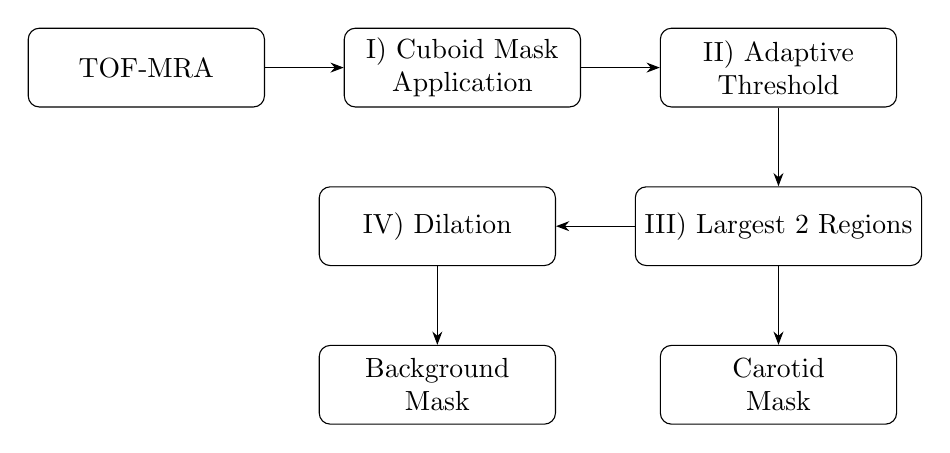
\begin{tikzpicture}[
			node distance=1cm,
			auto,
			>=Stealth,
			mybox/.style={draw, rounded corners, rectangle, minimum width=3cm, minimum height=1cm, align=center}
		]
		\node[mybox] (input) {TOF-MRA};
		\node[mybox, right=of input] (cuboid) {I) Cuboid Mask\\Application};

		\node[mybox, right=of cuboid] (thresh) {II) Adaptive\\ Threshold};
		\node[mybox, below=of thresh] (growing) {III) Largest 2 Regions};
		\node[mybox, left=of growing] (dilation) {IV) Dilation};
		\node[mybox, below=of growing] (mask) {Carotid\\Mask};
		\node[mybox, below=of dilation] (bg_mask) {Background\\Mask};

		\draw[->] (input) -- (cuboid);
		\draw[->] (cuboid) -- (thresh);
		\draw[->] (thresh) -- (growing);
		\draw[->] (growing) -- (mask);
		\draw[->] (growing) -- (dilation);
		\draw[->] (dilation) -- (bg_mask);
	\end{tikzpicture}
	\caption{Carotid and background mask segmentation pipeline}
	\label{fig:seg_pipeline}
\end{figure}

\section{Partial Volume Correction}

\subsection{Geometric Transfer Matrix}
% GPT: don't touch
As we discussed before in \ref{TODO}, direct extraction of the radioactivity in the arteries is not practical due to PVC.
Geometric Transfer Matrix aims to account for this loss of signal by considering the observed TACs are linear combination of the true value and other effecting regions \cite{rousset1998correction}.

Here we define two regions, the carotid and the surrounding tissues (background).
A mask for extracting the activities of the latter was obtained by dilating the carotid mask by 5 mm and subtracting the voxels corresponding to the carotid mask (Figure~\ref{fig:seg_pipeline}, Step IV).

\begin{equation}
	\underbrace{
		\begin{bmatrix}
			T_{c} \\
			T_{bg}
		\end{bmatrix}
	}_{\text{Observed}}
	=
	\underbrace{
		\begin{bmatrix}
			\omega_{c \rightarrow c}  & \omega_{bg \rightarrow c}  \\
			\omega_{c \rightarrow bg} & \omega_{bg \rightarrow bg}
		\end{bmatrix}
	}_{\text{GTM}}
	.
	\underbrace{
		\begin{bmatrix}
			T_{IF} \\
			T_{tissue}
		\end{bmatrix}
	}_{\text{Unknown}},
\end{equation}
where $\omega_{n \rightarrow m}$ are the spill-in and spill-over coefficient of region $n$ onto region $m$, which is obtained by convolving the binary mask of region $n$ with the system's point spread function and integrating the resulting intensity over region $m$, normalized by the total signal in region $m$.
where
\begin{equation}
	\omega_{n\to m} = \frac{\displaystyle \int_{\Omega_m} \bigl( h \ast \chi_n \bigr)(r)\,dr}{\displaystyle \int_{\Omega_m} \bigl( h \ast \chi_m \bigr)(r)\,dr},
\end{equation}
with \(\chi_n\) and \(\chi_m\) denoting the binary masks of regions \(n\) and \(m\), respectively, \(h\) the system's point spread function, and \(\Omega_m\) the spatial domain of region \(m\).

$T_{c}$ and $T_{bg}$ are respectively the observed carotid and background TACs and $T_{IF}$ and $T_{tissue}$ are the real unknown TACs of the carotid (the input function) and the background tissue.

By inverting the GTM, this system of equations can be solved to recover the arterial and background TACs.
% GPT: correct sentencing and explaining
However, GTM and other classical PVC methods often fail to fully recover the lost signal because they simplify the problem and ignore time-varying noise characteristics.
As a result, they may propagate or even amplify noise.
Time-varying noise arises from several factors, including the small diameter of the ICAs, very short early frames when the IF changes rapidly, and the exponential decay of the tracer, all of which reduce gamma counts detection by the PET camera and increase variance.

\subsection{Bayesian Geometric Transfer Matrix}

\subsubsection{Modelling}
% GPT: improve sentencing
For each subject, \(T_{IF}\) is modeled as a linear combination of a population mean and principal components obtained by applying principal component analysis (PCA) to AIFs from the cohort.
Specifically, for each subject, a subset randomly selected subjects—excluding the subject under study—is used to build a PCA basis.
After zero-centering the training AIFs, PCA yields principal axes \(\phi_i(t)\) with explained variances \(\lambda_i\).
We define scaled components \(v_i(t) = \sqrt{\lambda_i}\,\phi_i(t)\), and write
\begin{equation}
	T_{IF}(t) = \mu_{IF}(t) + \sum_{i=1}^p \theta_i\,v_i(t),
\end{equation}
where \(\mu_{IF}(t)\) is the population mean and the coefficients satisfy \(\theta_i \sim \mathcal{N}(0,1)\) by construction.
Here, \(p\) denotes the number of retained components.

% GPT: i dont like the sentencing and explanation at all
% Spectral Analysis (SA) describes tissue activity as a sum of exponential impulse responses convolved with the input function \cite{TODO}.
% It represents a flexible, linear decomposition of kinetics without committing to a specific compartmental topology, which is helpful for background tissue surrounding the ICAs.
%
Spectral analysis (SA) models tissue activity as the convolution of the input function with an impulse response written as a sum of exponentials \cite{TODO}.
This makes it more flexible and generalizable as it does not assume a particular compartment model and is convenient for describing background signal.
Therefore, the background TAC is

\begin{equation}
	T_{bg}(t) = \sum_{i=1}^s \alpha_{i} \,\bigl(T_{IF} \circledast e^{-\beta_{i} t}\bigr)(t),
\end{equation}
where \(\circledast\) denotes convolution, \(\alpha_i\) is the amplitude, and \(\beta_i\) is the decay rate of the \(i\)th spectral component.

\subsubsection{Noise}
% GPT: i dont like the sentencing and explanation at all
Accurate noise modeling is challenging because multiple sources contribute to the variance.
Some effects (e.g. scatter, randoms, and motion) are partially corrected during reconstruction post-processing.
The main contributor is low-count statistics, an inherent limitation of PET due to detector performance and overall camera sensitivity, which is particularly problematic for IDIF because the ICAs are small, early frames are very short during the bolus passage, and radioactive decay reduces detected events, increasing variance across frames.

While raw PET counts are Poisson-distributed, post-reconstruction noise is typically approximated as Gaussian \cite{TODO}.
To account for time-varying noise, we use per-frame weights to normalize variance across frames:
\begin{equation}
	\omega_{i} = \frac{\Delta t_i}{c_i}\,\exp\!\left(-\frac{t_{i}\,\ln 2}{T_{1/2}}\right),
\end{equation}
where \(\Delta t_i\) is the frame duration, \(c_i\) is the net true counts for frame \(i\), and \(T_{1/2}\) is the tracer half-life.
Because \(c_i\) was unavailable, we substitute \(C_T(t_i)\), the total reconstructed activity concentration at the frame mid-time.

The time-varying noise level is summarized by a weighted average variance:
\begin{equation}
	\sigma^2 = \frac{1}{N} \sum_{i=1}^{N} \omega_i\,\sigma_i^2.
\end{equation}

\subsubsection{Estimation}
% GPT: correct sentencing
Let \(\mathcal{D}\) denote the observed PET TAC, and let \( \Theta = (\theta_{1}, \dots,\theta_{p}, \alpha_{1}, \beta_{1}, \dots, \alpha_{s}, \beta_{s}) \) be the unknown model parameters, with an unknown Gaussian noise variance \(\sigma^2\).
We aim to estimate the joint posterior \(p(\Theta,\sigma^2\mid \mathcal{D})\).

By Bayes’ rule,
\begin{equation}
	p(\Theta,\sigma^2 \mid \mathcal{D}) \propto p(\mathcal{D} \mid \Theta,\sigma^2)\,\pi( \Theta )\,\pi( \sigma^2),
\end{equation}
where \(p(\mathcal{D} \mid \Theta,\sigma^2)\) is the likelihood and \(\pi(\cdot)\) are the priors.
We can therefore sample the posterior once the likelihood and priors are obtained.

The observed data are linked to the latent TACs through GTM \ref{TODO}.
For convenience, define
\begin{equation}
	\mathcal{T}(t) = \mathcal{G}(t;\Theta) =
	\mathcal{G}\!\left(
	\begin{bmatrix}
			T_{IF}(t;\theta_{1}, \dots, \theta_{p}) \\
			T_{tissue}(t;\alpha_{1}, \beta_{1}, \dots)
		\end{bmatrix}\right),
\end{equation}
where \(\mathcal{G}\) is the GTM operator and \(\mathcal{T}\) is the predicted activity (after PVE).
Assuming Gaussian noise with frame weights \(\omega_i\), the likelihood is
\begin{equation}
	p(\mathcal{D} \mid \Theta,\sigma^2) = \prod_{i=1}^N \frac{1}{\sqrt{2\pi \sigma^2}} \exp\!\left( -\frac{\omega_i\,\bigl(\mathcal{D}(t_i) - \mathcal{T}(t_i)\bigr)^2}{2\sigma^2} \right).
\end{equation}
We refer to this framework as the Bayesian Geometric Transfer Matrix (Bayesian GTM or BGTM).

The prior factorizes as
\begin{equation}
	\pi(\Theta) = \prod_{i=1}^p \pi(\theta_i)\,\prod_{j=1}^s \pi(\alpha_j)\,\pi(\beta_j).
\end{equation}
As noted above, \(\theta_i \sim \mathcal{N}(0,1)\).
For the spectral parameters, we adopt broad uniform priors,
\begin{equation}
	\alpha_i,\beta_i \sim \mathcal{U}( u_{\text{min}} , u_{\text{max}} ).
\end{equation}

For the noise variance, we use an inverse-gamma prior, \(\pi(\sigma^2) \sim \Gamma^{-1}(a_0,b_0)\), conjugate to the Gaussian likelihood.
We center this prior around an empirical weighted mean squared deviation between the observed carotid TAC and the mean AIF:
\begin{equation}
	\mathbb{E}[X] = \frac{1}{N} \sum_{i=1}^{N} \omega_i\,\bigl(T_c(t_i) - \mu_{IF}(t_i)\bigr)^2.
\end{equation}
Given a chosen coefficient of variation (CV), we set
\begin{equation}
	a_0 = 2 + \frac{1}{\mathrm{CV}^2}, \qquad b_0 = (a_0 - 1)\,\mathbb{E}[X].
\end{equation}

\subsubsection{Sampling}
% GPT: correct sentencing
Direct evaluation of the posterior \ref{TODO} is intractable, so we employ Monte Carlo sampling.
We use a Markov chain Monte Carlo scheme with a Metropolis-within-Gibbs strategy.

Gibbs updates draw each parameter from its univariate conditional posterior \(p(\Theta_i \mid \mathcal{D}, \Theta_{-i}, \sigma^2)\) and the noise variance from \(p(\sigma^2 \mid \mathcal{D},\Theta)\).
Metropolis–Hastings proposals explore \(\Theta\): at iteration \(m\), propose \(\Theta_{i}^\prime = \Theta_{i}^{(m)} + \varepsilon_{i}\,b\), where \(\varepsilon_i\) is the step size and \(b\) is a Brownian perturbation.
Accept with probability
\begin{equation}
	\min\!\left(1,\ \frac{p(\Theta_i^\prime \mid \mathcal{D}, \Theta_{-i}, \sigma^2)}{p(\Theta_i^{(m)} \mid \mathcal{D}, \Theta_{-i}, \sigma^2)}\right).
\end{equation}

Because the inverse-gamma prior is conjugate, the conditional posterior for \(\sigma^2\) is also inverse-gamma,
\begin{equation}
	p(\sigma^2 \mid \mathcal{D},\Theta) \sim \Gamma^{-1}(a, b),
\end{equation}
with
\begin{equation}
	a = a_0 + \frac{N}{2}, \qquad b = b_0 + \frac{1}{2}\sum_{i=1}^{N} \omega_i\,\bigl(\mathcal{D}(t_i) - \mathcal{T}(t_i)\bigr)^2.
\end{equation}
Thus, \(\sigma^2\) can be sampled directly without Metropolis–Hastings.

To improve mixing, each parameter \(k\) has its own proposal step size \(\epsilon_k\).
During burn-in, step sizes are adapted every \(L=50\) Metropolis–Hastings updates by an arbitrary acceptance rate of 0.5: if the empirical rate exceeds 0.5, increase \(\epsilon_k \leftarrow 1.1\,\epsilon_k\); otherwise decrease \(\epsilon_k \leftarrow 0.9\,\epsilon_k\).
After burn-in, step sizes are fixed and subsequent samples are retained.

\subsubsection{Inference}
% GPT: correct sentencing
After sufficient sampling, we use a modified maximum a posteriori (MAP) estimate by averaging the parameters of the top 0.1\% of samples ranked by posterior probability and reporting this average as the solution.
\section{Plasma Fraction Correction}
By construction, IDIFs extracted from PET represent whole-blood activity.
For \fdg, plasma metabolites are generally negligible over the scan, so the whole-blood AIF was used without plasma or metabolite correction \cite{TODO}.
For \yohimbine, kinetic modeling requires the plasma parent activity, so whole-blood IDIFs were converted to plasma and corrected for metabolites using
\begin{equation}
	C_{P,\mathrm{parent}}(t) \;=\; \frac{C_{WB,\mathrm{IDIF}}(t)}{R_{bp}} \,\times\, \mathrm{PPF}(t),
\end{equation}
where \(R_{bp}=0.661\) is the whole-blood–to–plasma ratio and \(\mathrm{PPF}(t)\) is the plasma parent fraction modeled as a 3 exponential curve:  \cite{TODO}
\begin{equation}
	\mathrm{PPF}(t) \;=\; 0.30\,e^{-t/0.88} \;+\; 0.09\,e^{-t/11.49} \;+\; 0.61\,e^{-t/65.77}.
\end{equation}
Because \(V_T\) estimation uses total plasma parent activity, no additional free-fraction correction was applied.

\section{Evaluation}

\subsection{IF Curves}
% GPT: Don't touch
The performance of the proposed IDIF estimation was first evaluated by computing the mean absolute error (MAE) between the cumulative area under the curve (cAUC) of the estimated IDIF and the \textit{ground true} AIF. cAUC was considered to be a more suitable metric since it provides an integrated measure of tracer exposure over time and is less sensitive to local fluctuations or noise in the curve compared to the directly comparing the TACs.
\begin{equation}
	\textrm{cAUC}(t) =  \int_{0}^{t} IF(\tau) \, d\tau,
\end{equation}
where \(IF\) is the input function.

\subsection{Quantification}
However, because the cAUC error does not fully capture the impact of IDIF deviations on kinetic parameters, absolute quantification was also performed to evaluate the performance of the estimated IDIF against the gold standard AIF.
Quantification was performed using graphical methods implemented in TPCCLIB \cite{oikonen2018tpcclib}.
The Patlak plot was used for \fdg\ \cite{patlak1983graphical}, and the Logan plot for \yohimbine\ \cite{logan1990graphical}.

The brain atlas was applied to the PET image and regional TACs were obtained by averaging voxels over time.
For \fdg, regional \(\mrglu\) was computed.
The mean absolute percentage error (MAPE) of \(\textrm{MR}_{\textrm{glu}}\) in each ROI was then calculated and averaged across the dataset:
\begin{equation}
	\text{Average MAPE}(\mrglu)= \frac{100}{N} \sum_{i=1}^{N} \left( \frac{1}{N_{\text{ROI}}} \sum_{j=1}^{N_{\text{ROI}}} \left| \frac{\textrm{MR}_{\textrm{glu},ij}^{\textrm{IDIF}} - \textrm{MR}_{\textrm{glu},ij}^{\textrm{AIF}}}{\textrm{MR}_{\textrm{glu},ij}^{\textrm{AIF}}} \right| \right),
\end{equation}
where \(N\) is the number of subjects.

Similarly, for \yohimbine, the volume of distribution (\(V_T\)) was calculated and the dataset error was computed as
\begin{equation}
	\mathrm{MAPE}(V_T)
	= \frac{100}{N}
	\sum_{i=1}^{N}
	\biggl(
	\frac{1}{N_{\mathrm{ROI}}}
	\sum_{j=1}^{N_{\mathrm{ROI}}}
	\left|
	\frac{V_{T,ij}^{\mathrm{IDIF}} - V_{T,ij}^{\mathrm{AIF}}}
	{V_{T,ij}^{\mathrm{AIF}}}
	\right|
	\biggr).
\end{equation}

Additionally, linear least-squares regression was performed between the regional \(\mrglu\) and \(V_T\) obtained using AIF and IDIF for each subject.
The coefficient of determination (\(R^2\)) and regression slope (\(S\)) were computed per subject.
The mean absolute percentage errors of these metrics across the dataset are
\begin{equation}
	\text{MAPE}(R^2) = \frac{100}{N} \sum_{i=1}^{N} \left| R^2_i - 1 \right|
\end{equation}
and
\begin{equation}
	\text{MAPE}(S) = \frac{100}{N} \sum_{i=1}^{N} \left| S_i - 1 \right|,
\end{equation}
where \(R^2_i\) and \(S_i\) denote the coefficient of determination and slope for subject \(i\), respectively.

\section{Simulation}
% GPT: fix coherence and sentencing
PET simulations are integral to validating statistical and analytical PET methods because they provide ground truth that may be unavailable or affected by human or instrumental error in experimental data.
In the previous section, we treated the AIF as the ground truth and evaluated methods against it.
However, because AIF measurement and analysis involve multiple manual steps and devices operated by different personnel, errors can occur.

Therefore, as a complementary validation, we conducted realistic simulations and evaluated the method on these data as well.
PET-SORTEO is a Monte Carlo PET simulation platform \cite{TODO} whose accuracy has been validated repeatedly \cite{TODO,TODO} and can closely approximate real acquisitions.
This fidelity strongly depends on accurate descriptions of both the physical anatomy and tracer kinetics.

As input, PET-SORTEO requires the description and characteristics of the PET machine, a 3D emission phantom segmenting the tissues into emitting regions, a 3D attenuation phantom describing tissue attenuation coefficients, and TACs for each emitting region.
For this study, we simulated the \fdg\ dataset using the Biograph mMR model to mirror the experimental datasets, and we derived numerical phantoms and TACs from the real MR and PET data.

For each subject, first, the brain atlas subregions were merged into larger regions: white matter (WM), gray matter (GM), gray nuclei (GN), cerebellar gray matter (CGM), and cerebellar white matter (CWM).
An algorithm originally developed for pseudo-CT generation from T1-weighted MRI for bone attenuation correction was used to create masks for the extracerebral regions\cite{TODO}.
Values above 300 were labeled as bone (BONE) and values between \(-300\) and \(300\) after excluding the brain as extracerebral soft tissues (SOFT) which includes the scalp, neck muscles, glands, eyes, etc.
The leftover space between the skull and the brain was labeled as cerebrospinal fluid (CSF).
Finally, the arterial mask (ICA) was obtained from the TOF-MRA segmentation (Section~\ref{sec:carotid}).
These nine regions were combined to form the emission phantom.

The attenuation phantom was generated from the pseudo-CT by segmenting SOFT and BONE and assigning their respective attenuation coefficients.

The emission phantom was then registered to PET space to extract subject-specific TACs.
These TACs were corrected for PVE using GTM and subsequently fitted with a 2TCM to denoise and obtain "ideal" TACs.
The AIF used for fitting was the subject’s measured AIF, itself fitted to an exponential model to remove noise \cite{feng}.

Several practical considerations were applied.
Our SOFT definition is broad; while adequate for simulation, it violates homogeneity assumptions in compartment modeling, so the unfitted TAC was retained for SOFT.
The pseudo-CT algorithm was permissive for BONE, leading to overestimated BONE TACs due to spill-in; empirically, BONE activity was scaled by 0.5.

Extracting the correct activity of the CSF with this approach is not feasible since it's a very thin region which is heavily affected by PVE. Thus, CSF TAC was considered 0.2 of the fitted WM TAC.
% The CSF is very thin in places and heavily affected by PVE, and GTM fails to correct it. Thus, CSF TAC was set to 0.2 of the fitted WM TAC.

\begin{tikzpicture}[
		node distance=1cm and 2cm,
		auto,
		>=Stealth,
		mybox/.style={draw, rounded corners, rectangle, minimum width=2cm, minimum height=1cm, align=center}
	]

	\node[mybox,minimum width=3cm] (pet) {PET};
	\node[mybox,minimum width=3cm, below=of pet] (t1) {T1w MRI};
	\node[anchor=south east] at($(pet.north)+(0,0.5)$) (pet_image) {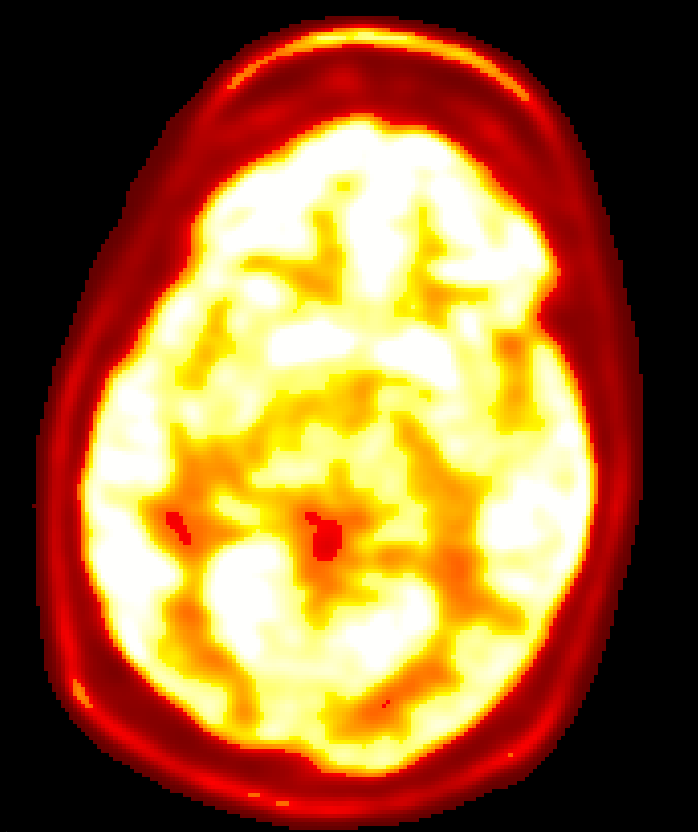
\includegraphics[height=3cm]{figures/real_pet.png}};
	\node[right=0.1cm of pet_image] (t1_image) {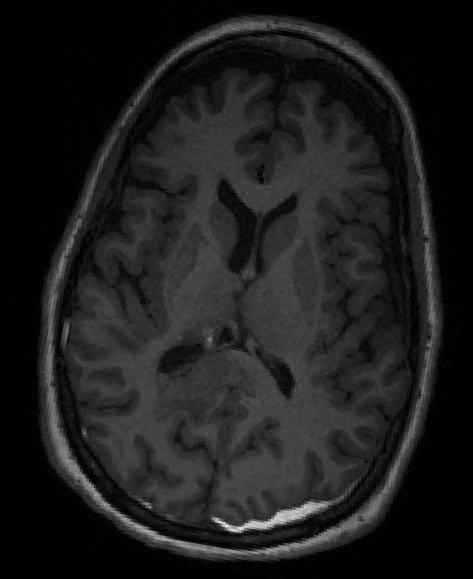
\includegraphics[height=3cm]{figures/t1.png}};


	\node[mybox, right=5cm of pet, minimum width=3cm] (ttac) {Tissue Activity};
	\node[mybox, right=5cm of t1, minimum width=3cm] (phantom) {Anatomical\\Phantom};

	\node[anchor=south east] at($(ttac.north)+(0,0.5)$) (phantom_image) {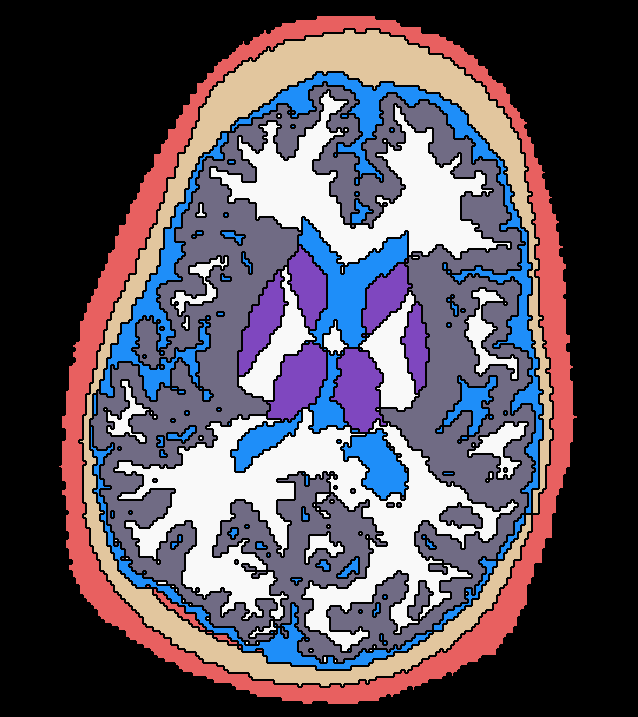
\includegraphics[height=3cm]{figures/phantom.png}};
	\node[right=0cm of phantom_image] (ttac_image) {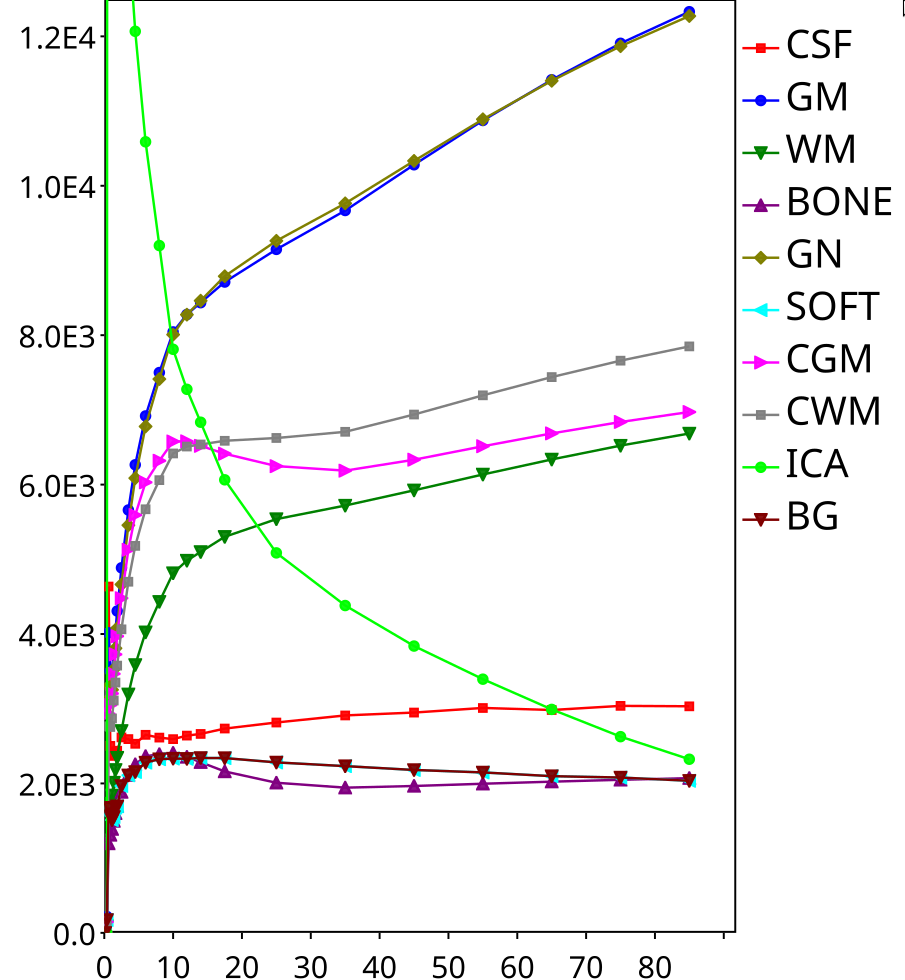
\includegraphics[height=2cm]{figures/ttacs.png}};

	\node[mybox, below=1.5cm of phantom, minimum width=3.3cm] (proto) {Simulation \\ Description Protocol};
	\node[below=0.5cm of proto] (phantom_image) {
\includegraphics[height=3cm]{figures/simulation_input_pet.png}};

	\node[mybox, below=1.7cm of t1, minimum width=3cm] (simpet) {Simulated PET};
	\node[below=0.5cm of simpet] (phantom_image) {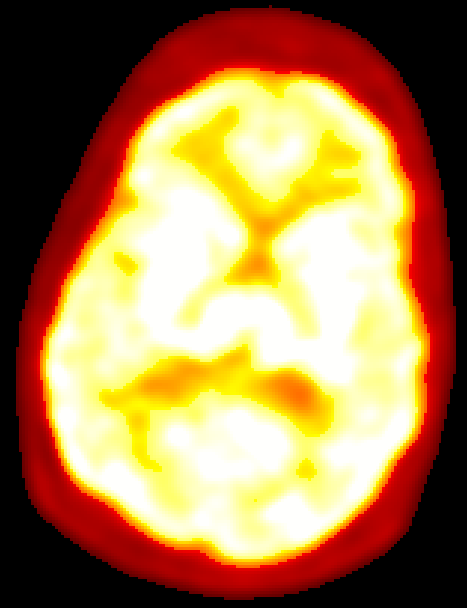
\includegraphics[height=3cm]{figures/simulated_pet.png}};

	\draw[->]
	(pet.east) to[out=0, in=180]
	node[yshift=+2pt, above] {\textit{Compartmental Fitting}}
	node[yshift=-2pt, below] {\textit{\& PVC}}
	(ttac.west);

	\draw[->]
	(t1.east) to[out=0, in=180]
	node[yshift=+2pt, above] {\textit{Tissue}}
	node[yshift=-2pt, below] {\textit{Classification}}
	(phantom.west);

	\draw[->] (ttac.east) to[out=0, in=0] (proto.east);

	\draw[->] (phantom.east) to[out=0, in=0] (proto.east);

	\draw[->]
	(proto.west) to[out=180, in=0]
	node[yshift=+2pt, above] {\textit{Monte Carlo}}
	node[yshift=-2pt, below] {\textit{Simulation}}
	(simpet.east);

	\begin{pgfonlayer}{background}
		\draw[dashed, rounded corners, thick]
		($(pet.north west)+(-0.3,0.3)$) rectangle ($(t1.south east)+(0.3,-0.3)$);
	\end{pgfonlayer}
	\node at ($(t1.south)-(0,0.5)$) {\text{Real Life Data}};

	\begin{pgfonlayer}{background}
		\draw[dashed, rounded corners, thick]
		($(ttac.north west)+(-0.3,0.3)$) rectangle ($(phantom.south east)+(0.3,-0.3)$);
	\end{pgfonlayer}
	\node at ($(phantom.south)-(0,0.5)$) {\text{Ground Truth}};
\end{tikzpicture}

\chapter{Results}
\section{Carotid Segmentation from MRA-TOF}
As illustrated in Figure~\ref{fig:seg_compare}, the cuboid mask plays a crucial role in the carotid segmentation.
Because no ground truth segmentation is available, visual inspection was used to evaluate the results.
% The measures described in Section~\ref{sec:carotid} significantly improved carotid segmentation by effectively excluding brain lesions and undesired venous structures.
% , which showed that lesions and venous structures were rarely selected by the algorithm.
% However, the algorithm acted overly conservative at times. It inadvertently excluded the periphery of the larger vessels or completely excluded the narrow ones.
\begin{figure}[h]
	\centering
	\begin{subfigure}{0.45\textwidth}
		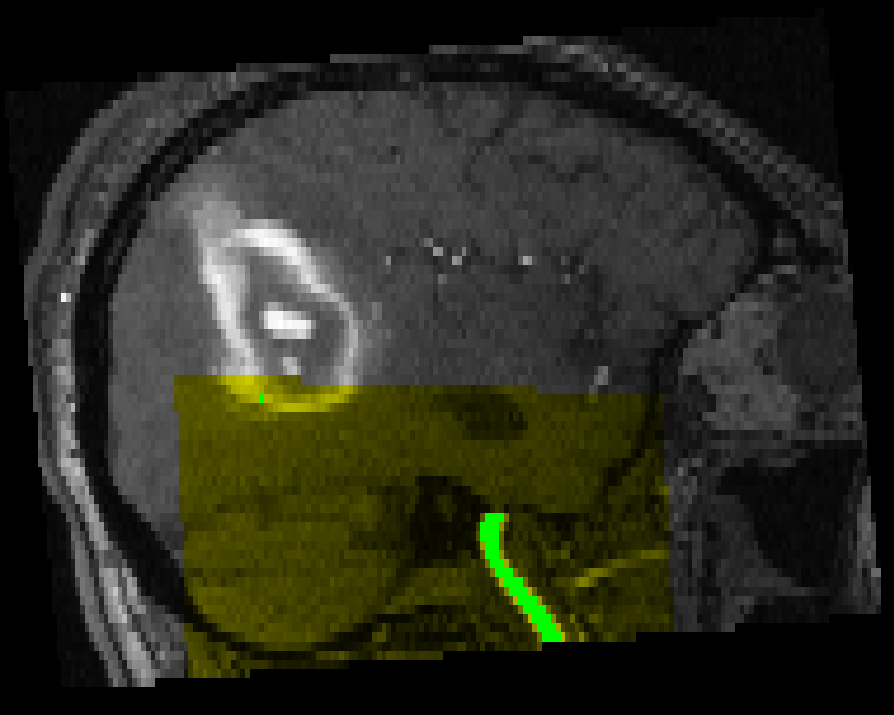
\includegraphics[width=\textwidth]{figures/molgu07704_bbox.png}
		\caption{}
		\label{subfig:seg_bbox}
	\end{subfigure}
	\begin{subfigure}{0.45\textwidth}
		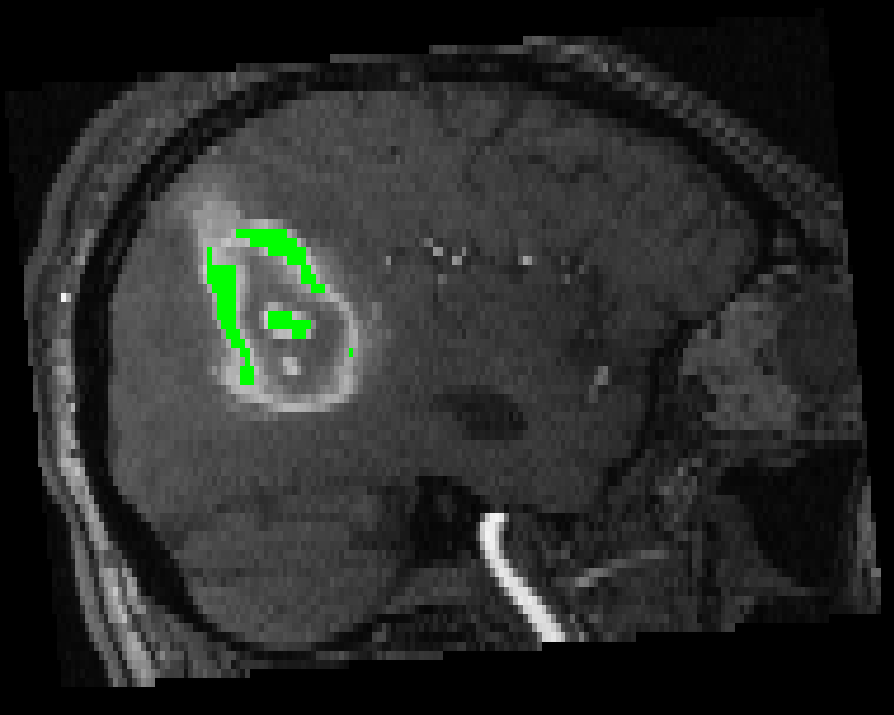
\includegraphics[width=\textwidth]{figures/molgu07704_nobbox.png}
		\caption{}
		\label{subfig:seg_nobbox}
	\end{subfigure}
	\caption{Comparison of carotid segmentation (green) with (a) and without (b) a cuboid mask (yellow). In the absence of the cuboid mask, the segmentation algorithm fails to capture the carotid and instead incorrectly identifies the brain lesion}
	\label{fig:seg_compare}
\end{figure}

\section{Hyperparameter Tuning}

The number of principle components $p$ was chosen as 3 by analysing the explained variance ratio plot in Figure~\ref{TODO}.
We see with only 3 components we get more than 90\% explained variability.
To prove the availability of the method, we seek to find the lowest possible number of population needed for the PCA in our \fdg $\,$ dataset.
To do this, the experiment was repeated 10 times each time with a different random seed for choosing population for $N=\{5,10,20,30,40,60\}$ and the resulting quantification errors were averaged.
As apparent in Figure~\ref{TODO}, we see a plateau in the performance after $N=10$ [TODO] and it was chosen as the ideal population sample count.
For the \yohimbine$\,$ dataset since it only has 7 subjects, $N=6$ was chosen.

In model fitting using SA, an appropriate spectral range is chosen based on the radioisotope half-life (e.g. $10^{-4} \mathrm{s}^{-1}$ to $1 \mathrm{s}^{-1}$ for $^{18}\mathrm{F}$ ) and is then divided in to $s=100$ or $s=1000$ fixed frequencies ($\beta$) then their amplitudes ($\alpha$) are fitted to the TAC \ref{TODO}.
The peaks in the resulting spectrum are considered as the [TODO] frequencies of the TAC.
However, estimating 100 or 1000 different amplitude parameters using MCMC would not be computationally feasible.
Instead we must chose an appropriate number of spectral components and let the model to tune the frequencies and the amplitudes together.

To derive the number of basis functions, we assumed the activity in the surrounding tissue can either be modelled as 1TCM or 2TCM which their Impulse Response Function (IRF) have respectively one and two basis functions.
Experiments with two basis functions showed that the model rarely results in two distinctive frequencies and would generally converge to similar values for both frequencies.
Thus for both datasets one basis function was chosen.

As discussed in Section~\ref{TODO}, the prior distribution used for the PCA weighting coefficients was $\theta_i \sim \mathcal{N}(0,1)$.
The prior for the SA parameters were considered a very uninformative uniform distribution $\mathcal{U}(10^{-5},10^{-2})$ as we did not have concrete prior knowledge on these parameters.


\section{Simulation}
From the 59 subjects in the \fdg $\,$ dataset, 24 subjects were excluded due to having very large brain tumors or opened skulls due to open brain surgery which caused the tissue classification algorithm to fail.
The rest of the 35 subjects were used to create the numerical phantoms and to generate TACs for the simulations.
Although the point of the simulation was not to replicate the same subject exactly but only use it as an inspiration for what real TACs look like, the results of the simulations were compared to the real scans as a quality control step.
In Figure~\ref{TODO} we see the 2nd and last frame axial [TODO] view of the real PET, the simulation input, and the simulation output.
As expected we see less details in the neck area (SOFT region) since we did not consider the complete arterial and venous structure as well as glands. But more importantly, we can clearly see the activity in the internal carotids.
In the last frame we can also see the activity of the brain to be very realistic.

However, the 



\section{IDIF}

Since BGTM relies on the GTM method and also depends on a population AIF. Thus the performance should be compared compared to the IDIF derived from GTM method and also the Population Based Input Function (PBIF) which is the mean AIF used in the PCA.


Figure~\ref{fig:ifs} compares the two methods for one of the best- and worst-performing subjects.
In the well-performing subject, BGTM significantly outperforms GTM ($\mrglu$ MAPE of 3.1\% vs. 20.9\%); however, in the poorly performing case, BGTM falls short of GTM ($\mrglu$ MAPE of 31.4\% vs. 19.5\%).
The average mean absolute error of the cAUC curves across the dataset was 14,202 for BGTM and 33,764 for GTM (Figure~\ref{subfig:cauc_boxplot}).

\begin{figure}[h]
	\centering
	\begin{subfigure}[b]{0.322\textwidth}
		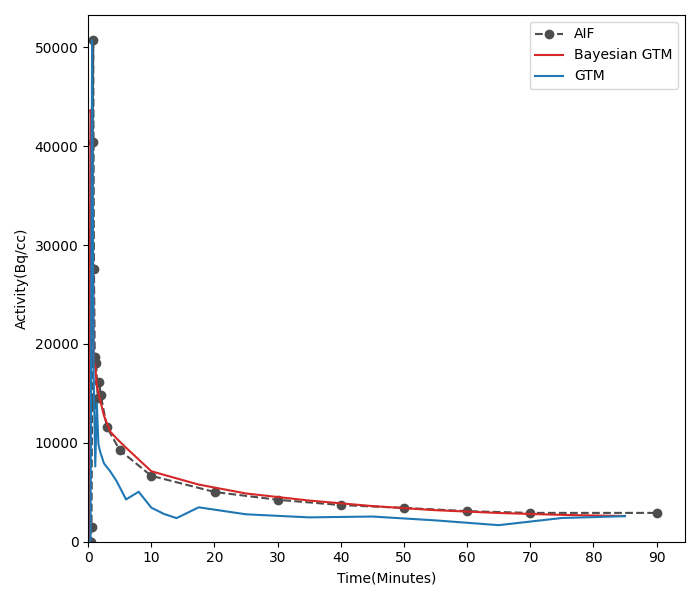
\includegraphics[width=\textwidth]{figures/MOLGU07704_1_if_comparison.png}
		\caption{}
		\label{subfig:good_if_compare}
	\end{subfigure}
	\begin{subfigure}[b]{0.322\textwidth}
		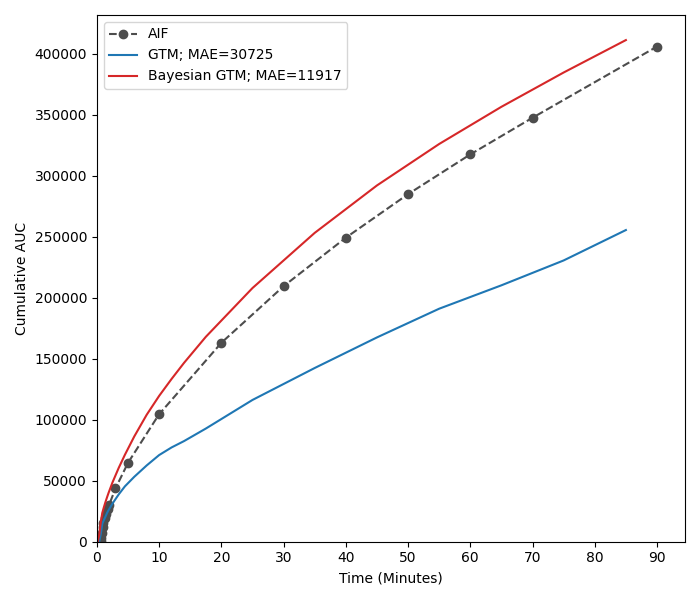
\includegraphics[width=\textwidth]{figures/MOLGU07704_1_trap.png}
		\caption{}
		\label{subfig:good_trap_compare}
	\end{subfigure}
	\begin{subfigure}[b]{0.322\textwidth}
		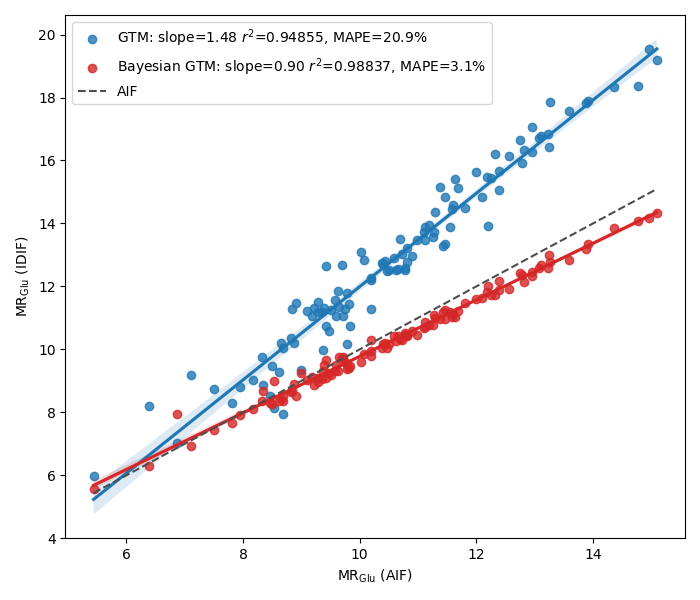
\includegraphics[width=\textwidth]{figures/MOLGU07704_1_cmrglu.png}
		\caption{}
		\label{fig:good_cmrglu}
	\end{subfigure}
	\begin{subfigure}[b]{0.322\textwidth}
		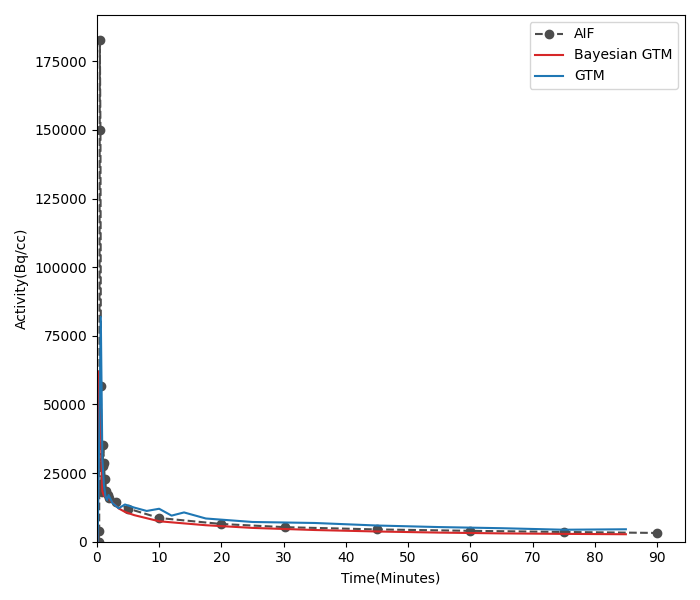
\includegraphics[width=\textwidth]{figures/CM10250_1_if_comparison.png}
		\caption{}
		\label{subfig:bad_if_compare}
	\end{subfigure}
	\begin{subfigure}[b]{0.322\textwidth}
		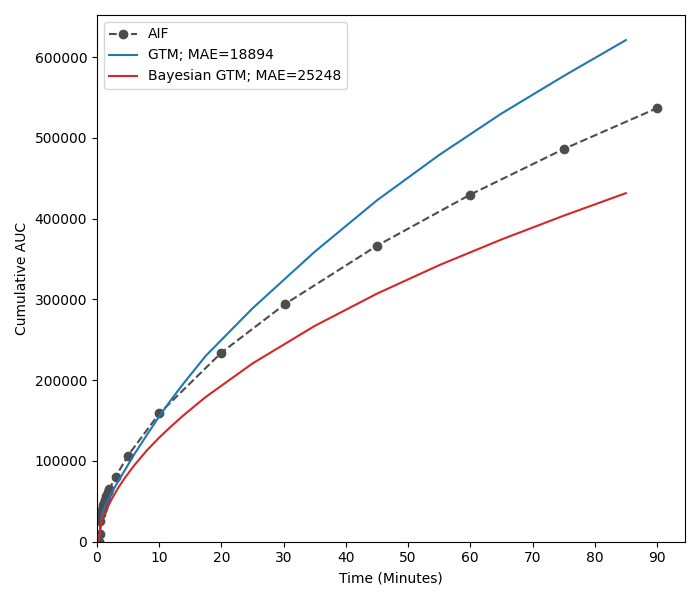
\includegraphics[width=\textwidth]{figures/CM10250_1_trap.png}
		\caption{}
		\label{subfig:bad_trap_compare}
	\end{subfigure}
	\begin{subfigure}[b]{0.322\textwidth}
		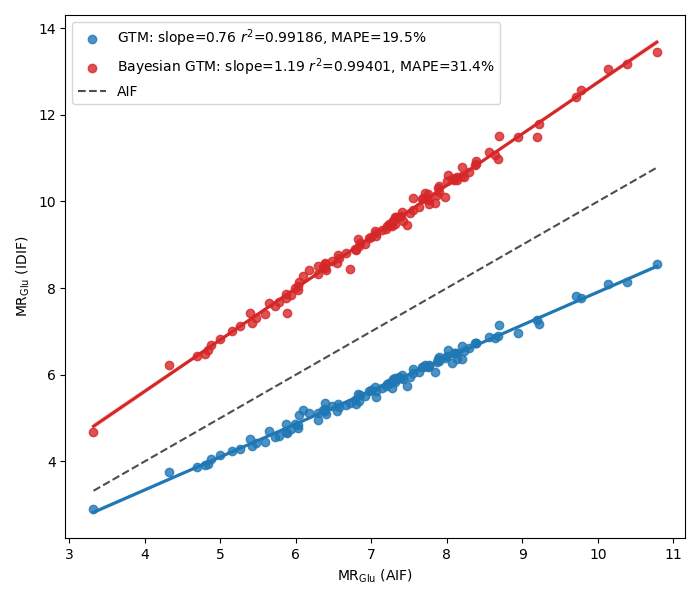
\includegraphics[width=\textwidth]{figures/CM10250_1_cmrglu.png}
		\caption{}
		\label{fig:bad_cmrglu}
	\end{subfigure}
	\caption{Comparison of the IFs (a,d), cumulative AUC curves (b,e), and $\mrglu$ regression lines (c,f) for one of the best-(top row) and worst-performingr(bottom row) subjects}
	\label{fig:ifs}
\end{figure}

ROI-based quantification was carried out using both IDIF methods, with BGTM yielding significantly better performance.
Specifically, the BGTM and GTM methods achieved an average \(\mrglu\) mean absolute percentage error (MAPE) of 14.1\% and 33\%, respectively (Figure~\ref{subfig:mape_boxplot}), and an average \(\mrglu\) MAE of 1.42 and 3.5.
In addition, the MAE for the coefficient of determination (\(R^2\)) and the regression slope (\(S\)) were 0.004 and 0.14 for BGTM, compared to 0.030 and 0.304 for GTM, respectively.

\begin{figure}
	\centering
	\begin{subfigure}[b]{0.45\textwidth}
		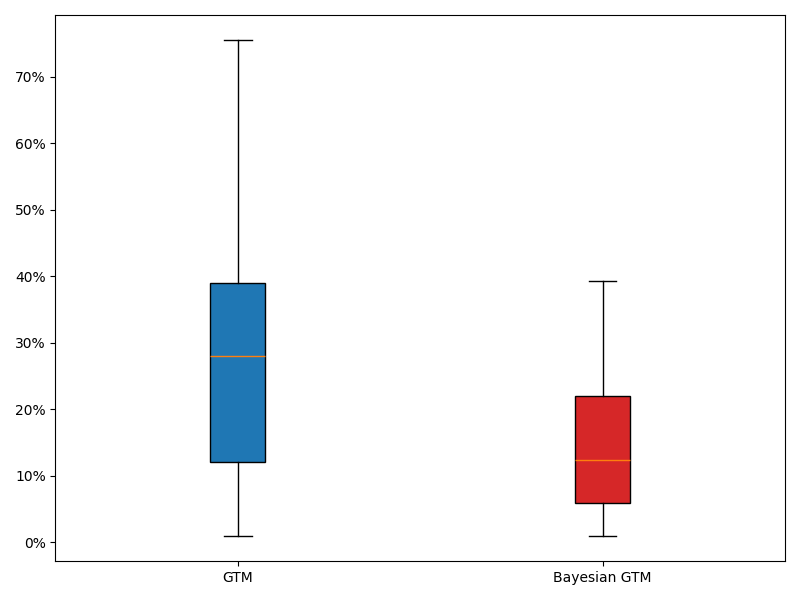
\includegraphics[width=\textwidth]{figures/quantification_mape_fitk3_boxplot.png}
		\caption{\(\mrglu\) MAPE Boxplot}
		\label{subfig:mape_boxplot}
	\end{subfigure}
	\begin{subfigure}[b]{0.45\textwidth}
		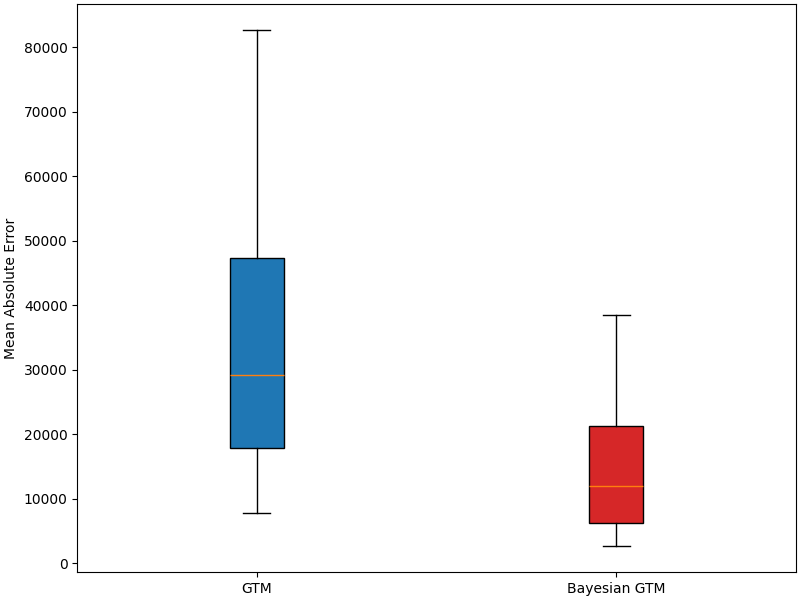
\includegraphics[width=\textwidth]{figures/curve_errors_boxplots.png}
		\caption{cAUC MAE Boxplot}
		\label{subfig:cauc_boxplot}
	\end{subfigure}
	\caption{Boxplot of curve and quantification errors}
	\label{fig:boxplots}
\end{figure}

\begin{table}[b]
	\centering
	\begin{tabular}{l|cc|cc|cc}
		\toprule
		\multirow{3}{*}{\textbf{Metric}} & \multicolumn{2}{c|}{\textbf{BGTM}} & \multicolumn{2}{c}{\textbf{GTM}} & \multicolumn{2}{c}{\textbf{Paired T-Test}}                                                 \\
		\cmidrule(lr){2-3} \cmidrule(lr){4-5} \cmidrule(lr){6-7}
		                                 & \(\mu\)                            & \(\sigma\)                       & \(\mu\)                                    & \(\sigma\) & T-Value & P-Value                \\
		\midrule
		IF cAUC MAE                      & 14,202                             & 9,190                            & 33,764                                     & 21,212     & 7.44    & \(7.2\times 10^{-10}\) \\
		$\mrglu$ MAPE (\%)               & 14.1                               & 10.1                             & 33.0                                       & 31.5       & 4.32    & \(6.5\times 10^{-5}\)  \\
		$\mrglu$ MAE                     & 1.42                               & 1.07                             & 3.50                                       & 3.38       & 4.41    & \(4.8\times 10^{-5}\)  \\
		$\mrglu$ \(R^2\) MAE             & 0.004                              & 0.006                            & 0.030                                      & 0.132      & 1.45    & \(1.5\times 10^{-1}\)  \\
		$\mrglu$ Slope MAE               & 0.14                               & 0.109                            & 0.304                                      & 0.230      & 4.73    & \(1.6\times 10^{-5}\)  \\
		\bottomrule
	\end{tabular}
	\caption{Summary of performance metrics for BGTM and GTM methods and their paired t-test.
		% $\mu$ is the average and $\sigma$ is the standard deviation
	}
	\label{tab:metrics}
\end{table}

A paired t-test was conducted to compare the performance of BGTM and GTM across previously mentioned metrics.
The results, summarized in Table~\ref{tab:metrics}, indicate that BGTM significantly outperforms GTM in cAUC MAE(\( t = 7.44 \), \( p = 7.2 \times 10^{-10} \)), $\mrglu$ MAPE (\( t = 4.32 \), \( p = 6.5 \times 10^{-5} \)), $\mrglu$ MAE (\( t = 4.41 \), \( p = 4.8 \times 10^{-5} \)), and $\mrglu$ Slope MAE (\( t = 4.73 \), \( p = 1.6 \times 10^{-5} \)), demonstrating the effectiveness of the proposed method.
However, no significant difference was observed in $\mrglu$ \(R^2\) MAE (\( t = 1.45 \), \( p = 0.15 \)).

As illustrated in Figure~\ref{fig:corr_mat}, there is a strong correlation between the cAUC MAE and the quantification errors suggesting cAUC as a reliable intermediate metric.

\begin{figure}[h]
	\centering
	\begin{subfigure}{0.45\textwidth}
		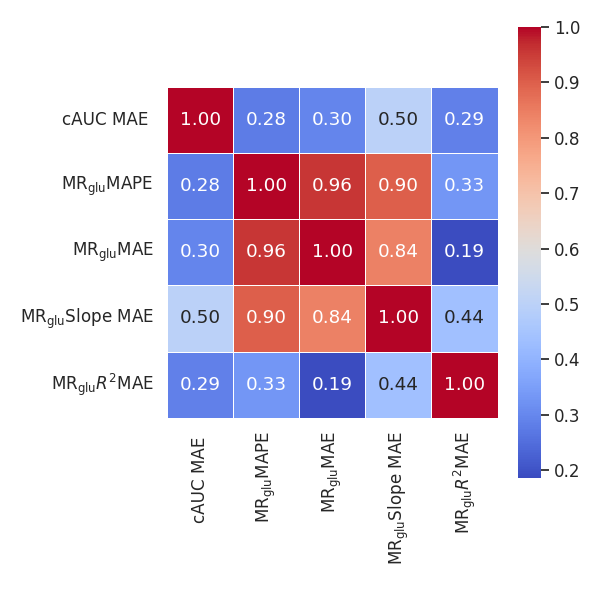
\includegraphics[width=\textwidth]{figures/corr_gtm.png}
		\caption{GTM}
		\label{subfig:corr_gtm}
	\end{subfigure}
	\begin{subfigure}{0.45\textwidth}
		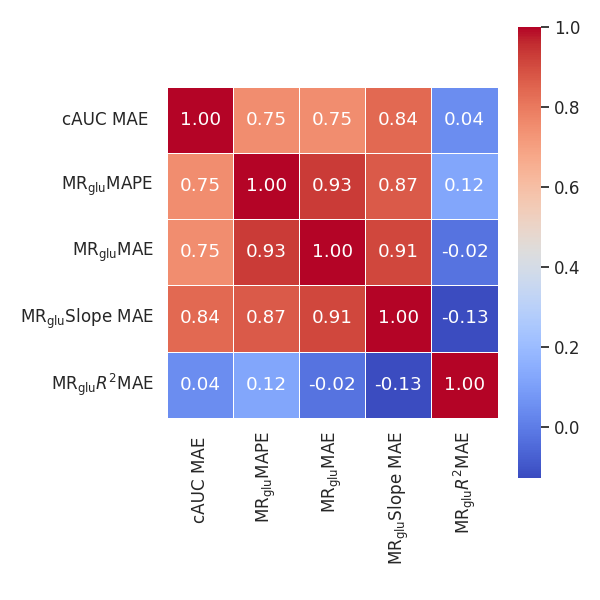
\includegraphics[width=\textwidth]{figures/corr_bgtm.png}
		\caption{Bayesian GTM}
		\label{subfig:corr_bgtm}
	\end{subfigure}
	\caption{Correlation matrix of different metrics for Bayesian GTM and GTM methods}
	\label{fig:corr_mat}
\end{figure}




\chapter{Discussion}

In this study, we sought to replace arterial sampling by estimating an image-derived input function (IDIF) from dynamic brain PET.
We used a Bayesian Markov chain Monte Carlo (MCMC) framework that we refer to as Bayesian GTM (BGTM).
BGTM models partial-volume effects and time-varying noise while jointly estimating the input function and the surrounding tissue activities.

Accurate IDIF requires a reliable segmentation of an artery.
We proposed a fast and fully automatic yet simple segmentation algorithm that extracts the internal carotid arteries from the TOF-MRA image.
We placed a simple cuboid mask over the expected ICA location, which allowed high-intensity thresholding to avoid non-arterial hyperintense tissues such as lesions.
Because no ground-truth labels were available, evaluation relied on visual inspection. Future work should include expert annotations to enable statistical metrics such as the Dice coefficient.
TOF-MRA is not routinely included in many imaging protocols, which limits its immediate applicability.

Spectral analysis was an appropriate choice for modeling the background tissue because it does not force a fixed kinetic model and is much more flexible.
A fixed one- or two-tissue model can be mismatched when regional kinetics do not follow those forms.
The input-function model used a PCA prior, which captured most of the variability with a few coefficients.
However, it still relies on a sufficiently large AIF population.
A parametric alternative such as the exponential model of \citeauthor{feng1993models} \cite{feng1993models} could reduce this dependence, provided tracer-specific informative priors on those parameters are available.

We treated noise as time-varying and used frame-wise weights to normalize variance across time frames.
Future work could estimate a separate noise level per frame rather than summarizing the variance with a single statistic.

Bayesian inference rests on the likelihood and the priors.
Thus, the quality and informativeness of the priors can drastically affect the results.
By nature, in the PCA-based input function, the coefficients have a strongly informative prior of \(\theta_i \sim \mathcal{N}(0,1)\).
If a parametric input function model such as Feng were used instead, parameters would need tracer-specific priors that encode the underlying kinetics.
One way to achieve this is to fit the parametric model to a population of AIFs and use the empirical parameter distributions as priors.
For the spectral model of background kinetics, we lacked informative prior knowledge and used wide uniform priors.
More informative priors could improve accuracy and robustness.

In the \fdg\ study, a larger PCA population was available, and the subjects were comatose, which likely reduced inter-subject variability due to low glucose uptake and also reduced motion artifacts.
These factors allowed for achieving a high performance by BGTM which was not replicated in the \yohimbine\ study.
This cohort was small and consisted of healthy young adults with greater inter-subject variability.
In addition, for this tracer, plasma parent correction was required and was applied with a population-based curve, which does not capture subject-specific metabolism.
These factors likely contributed to the weaker results.

We ran Monte Carlo PET simulations as a complementary evaluation step with the special advantage of controlled conditions and known ground truth.
The simulation protocol drew anatomy and kinetics from real scans to keep inputs realistic.
The goal was quality control of the pipeline rather than replication of individual scans, and comparisons to real data were used only as sanity checks.
As discussed in Section~\ref{sec:results_simulation}, regional activities were broadly in line with the real data, and Figure~\ref{fig:sim_compare_imgs} shows that early and late frames look consistent with the intended kinetics.
However, Figure~\ref{fig:sim_tac_compare} shows substantial bias in the Direct IDIF for simulated data compared to the experimental data.
Naturally, this bias then propagated into GTM and therefore BGTM, causing significantly worse performance compared to the experimental \fdg\ dataset.

Several factors could explain this bias.
First, for reasons pointed out in Section~\ref{sec:methods_simulation}, contrary to other regions, the TTAC of the SOFT region was taken raw from the experimental scan rather than fitting to a compartment model.
This caused the activity in the SOFT region to follow a different kinetic profile than the rest of the regions.
And since the background tissue lay inside the SOFT region, it affected its signal and therefore affected the ICA signal by spill-in.
A better approach would be to set plausible amplitudes and decay rates in an SA model for SOFT and generate its TACs from those parameters.
This also has the added advantage of being able to compare BGTM’s estimated spectral parameters with the known ground truth.
Second, we resampled PET-derived TTACs and the fitted AIF ICA curve to mid-frame times to match the experimental framing, which can lose temporal detail.
Third, the AIF was fitted with the Feng model using TPCCLIB, and some fits showed unrealistic peaks or fast recirculation, which can propagate bias to all IDIF methods.

To our knowledge, whole-brain Monte Carlo simulation with an explicit carotid input for IDIF validation has not been reported.
If the present simulation framework is refined, it could support systematic studies across key factors.
These factors include input-function shape (peak height, sharp versus broad peak, slow versus fast decay), background activity level, isotope, frame durations, and scanner geometry.
Studying these dimensions would clarify when IDIF methods are reliable, highlight failure modes, and guide improvements to the BGTM implementation to adapt to different studies.


\chapter{Conclusion}
 [TODO]

\section*{Prospects}
In this internship, I developed a deeper understanding and a strong interest in research in PET kinetic modelling and medical image processing.
Therefore, I will pursue a PhD at CERMEP under the supervision of Dr. Costes and Dr. Merida after completing this Master's program.
Funding was secured through the annual PhD fellowship competition of the Interdisciplinary Doctoral School of Health Sciences (L'École Doctorale Interdisciplinaire Sciences Santé, EDISS), in which I placed joint first.

The PhD is titled “Multimodal PET–MR Imaging: Dynamic Modelling of Neurotransmitter Release and Analysis of Neurovascular Coupling.”
The project aims to implement and validate a kinetic modelling method that enables detection and characterization of endogenous neurotransmitter release, in competition with a specific PET tracer (ntPET), and to link this release to neurovascular coupling measured with functional MRI.

At CERMEP, a Bayesian framework for estimating kinetic model parameters has been developed \cite{irace2020bayesian} which is actually the inspiration of the original BGTM implementation and this internship.
The performance of our approach has been evaluated on simulated data.
However, further work is required to develop a robust statistical model able to assess the likelihood associated with a discharge and improve the estimation by incorporating prior knowledge from functional MRI data.

\newpage
\fancyhead{}
\fancyhead[L]{\textsc{References}}
\printbibliography[
	heading=bibintoc,
	title={References}]



\end{document}

